\documentclass[12pt,a4paper]{amsart}
\usepackage[slovene]{babel}
\usepackage[utf8]{inputenc}
\usepackage{amsmath,amssymb,amsfonts}
\usepackage{url}
\usepackage[dvipsnames,usenames]{color}
\usepackage{graphicx}

\graphicspath{ {./images/} }
\textwidth 15cm
\textheight 24cm
\oddsidemargin.5cm
\evensidemargin.5cm
\topmargin-5mm
\addtolength{\footskip}{10pt}
\pagestyle{plain}
\overfullrule=15pt 
% ukazi za matematicna okolja
\theoremstyle{definition} % tekst napisan pokoncno
\newtheorem{definicija}{Definicija}[section]
\newtheorem{primer}[definicija]{Primer}
\newtheorem{opomba}[definicija]{Opomba}

\renewcommand\endprimer{\hfill$\diamondsuit$}

\theoremstyle{plain} % tekst napisan posevno
\newtheorem{lema}[definicija]{Lema}
\newtheorem{izrek}[definicija]{Izrek}
\newtheorem{trditev}[definicija]{Trditev}
\newtheorem{posledica}[definicija]{Posledica}

% za stevilske mnozice uporabi naslednje simbole
\newcommand{\R}{\mathbb R}
\newcommand{\N}{\mathbb N}
\newcommand{\Z}{\mathbb Z}
\newcommand{\C}{\mathbb C}
\newcommand{\Q}{\mathbb Q}

% ukaz za slovarsko geslo
\newlength{\odstavek}
\setlength{\odstavek}{\parindent}
\newcommand{\geslo}[2]{\noindent\textbf{#1}\hspace*{3mm}\hangindent=\parindent\hangafter=1 #2}


\newcommand{\imeavtorja}{Ana Marija Kravanja}
\newcommand{\naslovdela}{Min-Graph Equipartition Problem with Simulated Annealing}
\newcommand{\letnica}{2019} 

\begin{document}

% od tod do povzetka ne spreminjaj nicesar
\thispagestyle{empty}
\noindent{\large
UNIVERZA V LJUBLJANI\\[1mm]
FAKULTETA ZA MATEMATIKO IN FIZIKO\\[5mm]}
\vfill

\begin{center}{\large
{\bf \naslovdela}\\[10mm]
Ana Marija Kravanja, Urška Jeranko, Oskar Kregar}\\[1cm]

\end{center}
\vfill

\noindent{\large
Ljubljana, \letnica}
\pagebreak


\section{Osnovno o projektu}
V naši projektni nalogi bomo reševali problem deljenja grafa. Naš cilj je graf razdeliti na dva skoraj enaka dela tako, da je med tema nastalima deloma čim manj povezav. Najti tako delitev je težek problem, ki postane še težji, če moramo preveriti zelo veliko rešitev, da najdemo optimalno. Reševali ga bomo s požrešno metodo (Greedy Method) in metodo simuliranega ohlajanja (Simulated Annealing Heuristic) ter nato rešitve metod primerjali med sabo in jih preizkusili na različnih grafih (gosti, redki, naključni) pri različnih parametrih (temperatura, sosednja vozlišča). 

\section{Požrešna metoda}
Požrešna metoda je strategija, ki na vsakem posameznem koraku izbere optimalno rešitev s ciljem, da nas to privede do globalno optimalne rešitve. To pomeni, da algoritem izbere rešitev, ki je trenutno najboljša, vendar se pri tem ne ozira na posledice - ne gleda celotne slike. Težava te metode je, da na vsakem koraku izbere le lokalno najboljšo rešitev, samo upamo pa lahko, da je to tudi prava pot do globalnega optimuma. Pogosto torej sploh ne najde najboljše rešitve, povsem mogoče je celo, da nas pripelje do najslabše možne. \\

Naj bo $G=(V,E)$ enostaven graf, pri čemer je $V$ množica vozlišč in $E$ množica povezav. Naj bo število vozlišč enako $n$. Definirajmo delitev grafa na dve množici X in Y, pri čemer je $|X| = \lceil \frac{n}{2} \rceil$. Iskali bomo minimalno širino bisekcije, to je najmanjše število povezav med $X$ in $Y$ med vsemi možnimi delitvami.

\begin{definicija}
Naj bo $G=(V,E)$ enostaven graf in $X,Y \subseteq V$, tako da je $X \cap Y = \emptyset$ in $X \cup Y =V$.
\begin{itemize}
\item Za $x \in X$ označimo z $I(x)$ notranjo vrednost, to je šteilo povezav $(x,z) \in E;z\in X \backslash \{x\}$ . Analogno definiramo $I(y)$ za $y \in Y$.
\item Za $x \in X$ označimo z $O(x)$ zunanjo vrednost, to je šteilo povezav $(x,z) \in E;z\in Y $ . Analogno definiramo $O(y)$ za $y \in Y$.
\item Za $x \in X, y \in Y$ naj bo $\omega(x,y) := \begin{cases} 1,&\text{if} (x,y) \in E\\ 
0, &\text{sicer}\end{cases} $.
\item Za $x \in X, y \in Y$ naj bo $S(x,y):= O(x)-I(x)+O(y)-I(y)-2\omega(x,y)$.
\end{itemize}
\end{definicija}

\subsection{Algoritem požrešne metode}
Začnemo z naključno delitvijo vozlišč grafa na dve skoraj enako veliki množici. Algoritem zamenja dve vozlišči na različnih straneh (pri čemer se vse povezave ohranijo), če s tem dobimo boljšo bisekcijo (manjše število povezav med stranema) in se ustavi, ko to ni več možno. Pri menjavi notranje vrednosti postanejo zunanje in obratno, zato dobimo izboljšano bisekcijo le, če je $S(x,y)>0$.
\subsubsection{Algoritem 1} 
Vhodni podatki: Graf $G=(V,E), |V|=n$.
\begin{enumerate}
\item Izberemo neključno delitev $(X,Y)$.
\item Izberemo $x\in X, y\in Y$, tako da je $S(x,y)>0$.
\item Zamenjamo vozlišči $x$ in $y$.
\item Ponavljamo 2. in 3. korak, dokler ne obstajata več $x\in X, y\in Y$, da je $S(x,y)>0$.
\end{enumerate}
Izhodni podatki: delitev $(X,Y)$.

\section{Metoda simuliranega ohlajanja}
Algoritem se je v osnovi razvil zaradi procesa toplotne obdelave kovin. Različne materiale segrevamo oz. ohlajamo, da bi spremenili fizikalne lastnosti njihove notranje strukture. Ko se kovina enkrat ohladi, postane njena nova struktura fiksna in kovina tako obdrži pridobljene lastnosti. Pri simuliranem ohlajanju je temperatura naša spremenljivka, ki ponazarja toplotni proces. Na začetku temperaturo nastavimo na visoko vrednost in jo nato sčasoma nižamo, ko se algoritem izvaja. Na začetku, ko je temperatura nastavljena na visoko vrednost, algoritem pogosteje sprejema rešitve, ki so slabše od naše trenutne rešitve zato, da se izogne lokalnim optimumom, ki nas ne bodo pripeljali do globalnega optimuma. Z nižanjem temperature pa se niža tudi verjetnost, da bo algoritem izbiral slabše rešitve; postopoma se torej osredotoči na iskalno območje, na katerem upamo, da je mogoče najti rešitev blizu optimalne. Algoritem je zelo učinkovit pri iskanju rešitev, ki so blizu optimalne, za probleme velikih velikosti, ki vsebujejo številne lokalne optimume.

\subsection{Algoritem metode simuliranega ohlajanja}
Graf si definiramo analogno kot pri požrešni metodi. Za $S(x,y)>0$ zamenjamo vozlišči, če pa je $S(x,y)<0$, vozlišči zamenjamo z verjetnostjo $$P(x,y,t) = e^{\frac{S(x,y)}{t}}; t\ge 0$$

\subsubsection{Algoritem 2}
S $Q(Z)$ je označena funkcija, ki množici Z priredi neko kvaliteto, torej če je $Q(Z) >Q(R)$, pomeni, da je množica Z bolj ugodna za nadaljnjo obravnavo.
Za funkcijo $Q$ smo si v našem primeru izbrali $S(x,y)$, ki je definiran enako kot pri požrešni metodi. Torej če je $S(x,y)$ funkcija, kjer smo v množici $R$ zamenjali x in y in $S(a,b)$ množica $Z$, kjer ju nismo zamenjali in velja, da je $S(x,y) > S(a,b)$, potem z določeno verjetnostjo zamenjamo $R$ z $Z$. 
\begin{enumerate}
\item t= temperatura z visoko vrednostjo
\item Z= začetna delitev grafa na množici X in Y 
\item N= Z  naj predstavlja trenutno najboljšo rešitev
\item ponovi, dokler je N najboljša rešitev, nam je zmanjkalo časa ali pa je $t \leq 0$
\item 			R=delitev, kjer zamenjamo $x$ in $y$
\item 			če je $Q(R)>Q(Z)$ ali naključno število med 0 in 1 manjše od $P(x,y,t)$, potem je $S=R$
\item 			zmanjšamo t
\item 			če je $Q(Z)>Q(N)$ 
\item 				$N=Z$
\item vrni $N$		
\end{enumerate}


\section{Primeri}
Poglejmo si nekaj primerov delitve grafov. 

\begin{figure}[h]
    \centering
    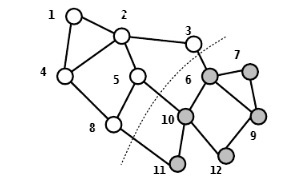
\includegraphics{prvi_graf} 
    \caption{primer grafa na 12 točkah}
    \label{fig:1_graf}
\end{figure}

\begin{figure}[h]
    \centering
    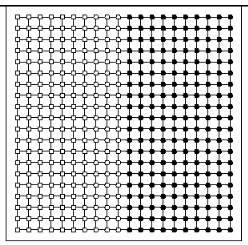
\includegraphics{drugi_graf} 
    \caption{primer grafa na 400 točkah, prikazana je optimalna rešitev}
    \label{fig:2_graf}
\end{figure}

\begin{figure}[h]
    \centering
    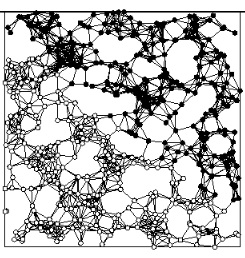
\includegraphics{tretji_graf} 
    \caption{Johnsonsov geometrični graf}
    \label{fig:3_graf}
\end{figure}


\end{document}
